% This is "sig-alternate.tex" V2.1 April 2013
% This file should be compiled with V2.5 of "sig-alternate.cls" May 2012
%
% This example file demonstrates the use of the 'sig-alternate.cls'
% V2.5 LaTeX2e document class file. It is for those submitting
% articles to ACM Conference Proceedings WHO DO NOT WISH TO
% STRICTLY ADHERE TO THE SIGS (PUBS-BOARD-ENDORSED) STYLE.
% The 'sig-alternate.cls' file will produce a similar-looking,
% albeit, 'tighter' paper resulting in, invariably, fewer pages.
%
% ----------------------------------------------------------------------------------------------------------------
% This .tex file (and associated .cls V2.5) produces:
%       1) The Permission Statement
%       2) The Conference (location) Info information
%       3) The Copyright Line with ACM data
%       4) NO page numbers
%
% as against the acm_proc_article-sp.cls file which
% DOES NOT produce 1) thru' 3) above.
%
% Using 'sig-alternate.cls' you have control, however, from within
% the source .tex file, over both the CopyrightYear
% (defaulted to 200X) and the ACM Copyright Data
% (defaulted to X-XXXXX-XX-X/XX/XX).
% e.g.
% \CopyrightYear{2007} will cause 2007 to appear in the copyright line.
% \crdata{0-12345-67-8/90/12} will cause 0-12345-67-8/90/12 to appear in the copyright line.
%
% ---------------------------------------------------------------------------------------------------------------
% This .tex source is an example which *does* use
% the .bib file (from which the .bbl file % is produced).
% REMEMBER HOWEVER: After having produced the .bbl file,
% and prior to final submission, you *NEED* to 'insert'
% your .bbl file into your source .tex file so as to provide
% ONE 'self-contained' source file.
%
% ================= IF YOU HAVE QUESTIONS =======================
% Questions regarding the SIGS styles, SIGS policies and
% procedures, Conferences etc. should be sent to
% Adrienne Griscti (griscti@acm.org)
%
% Technical questions _only_ to
% Gerald Murray (murray@hq.acm.org)
% ===============================================================
%
% For tracking purposes - this is V2.0 - May 2012



\documentclass{sig-alternate-05-2015}

\begin{document}

% Copyright
\setcopyright{acmcopyright}
%\setcopyright{acmlicensed}
%\setcopyright{rightsretained}
%\setcopyright{usgov}
%\setcopyright{usgovmixed}
%\setcopyright{cagov}
%\setcopyright{cagovmixed}


% DOI
\doi{10.475/123_4}

% ISBN
\isbn{123-4567-24-567/08/06}

%Conference
\conferenceinfo{PLDI '13}{June 16--19, 2013, Seattle, WA, USA}

\acmPrice{\$15.00}

%
% --- Author Metadata here ---
\conferenceinfo{WOODSTOCK}{'97 El Paso, Texas USA}
%\CopyrightYear{2007} % Allows default copyright year (20XX) to be over-ridden - IF NEED BE.
%\crdata{0-12345-67-8/90/01}  % Allows default copyright data (0-89791-88-6/97/05) to be over-ridden - IF NEED BE.
% --- End of Author Metadata ---

\title{ Mining HIV Trends in Social Media Data}
%
% You need the command \numberofauthors to handle the 'placement
% and alignment' of the authors beneath the title.
%
% For aesthetic reasons, we recommend 'three authors at a time'
% i.e. three 'name/affiliation blocks' be placed beneath the title.
%
% NOTE: You are NOT restricted in how many 'rows' of
% "name/affiliations" may appear. We just ask that you restrict
% the number of 'columns' to three.
%
% Because of the available 'opening page real-estate'
% we ask you to refrain from putting more than six authors
% (two rows with three columns) beneath the article title.
% More than six makes the first-page appear very cluttered indeed.
%
% Use the \alignauthor commands to handle the names
% and affiliations for an 'aesthetic maximum' of six authors.
% Add names, affiliations, addresses for
% the seventh etc. author(s) as the argument for the
% \additionalauthors command.
% These 'additional authors' will be output/set for you
% without further effort on your part as the last section in
% the body of your article BEFORE References or any Appendices.

\numberofauthors{2} %  in this sample file, there are a *total*
% of EIGHT authors. SIX appear on the 'first-page' (for formatting
% reasons) and the remaining two appear in the \additionalauthors section.
%
\author{
% You can go ahead and credit any number of authors here,
% e.g. one 'row of three' or two rows (consisting of one row of three
% and a second row of one, two or three).
%
% The command \alignauthor (no curly braces needed) should
% precede each author name, affiliation/snail-mail address and
% e-mail address. Additionally, tag each line of
% affiliation/address with \affaddr, and tag the
% e-mail address with \email.
%
% 1st. author
\alignauthor
Patrick Breen\\
       \affaddr{The Institute of Bioinformatics}\\
       \affaddr{The University of Georgia}\\
       \affaddr{Athens, Georgia}\\
       \email{pbreen@uga.edu}
% 2nd. author
\alignauthor
Shannon Quinn\titlenote{Corresponding author.}\\
       \affaddr{Institute of Computer Science}\\
       \affaddr{University of Georgia}\\
       \affaddr{Athens, Georgia}\\
       \email{squinn@cs.uga.edu}
}



\maketitle
\begin{abstract}

Here is the abstract.

\end{abstract}


%
% The code below should be generated by the tool at
% http://dl.acm.org/ccs.cfm
% Please copy and paste the code instead of the example below. 
%
% TODO: this section
\begin{CCSXML}

\end{CCSXML}


%
% End generated code
%

%
%  Use this command to print the description
%
\printccsdesc

% We no longer use \terms command
%\terms{Theory}

\keywords{ Social Media, Topic Modelling, Document Embedding}

\section{Introduction}

Introduce and literature review of:
1) PrEP, HIV, Twitter

 - social impact issues, efficacy, adherence issues, other STDs, Austin (Scott County) Indiana Outbreak as example
 
 - specifically other papers that did mining Twitter for HIV


2) Word2Vec, Doc2Vec

 - theory and application examples

3) Dynamic Topic models, Latent Dirichlet allocation

- theory and application examples

\section{Results}



We sought to determine trends in HIV and PrEP discourse on twitter, to inform and coordinate public health efforts to promote PrEP adoption and adherence for at-risk individuals. We collected 624,569 tweets related to 'HIV', 'AIDS', 'truvada', 'prophylaxis', 'imtesting', 'PrEP' from Twitter's streaming API. The tweets were restricted to English language, and the collection dates spanned from the 47th week of 2015 to the 14th week of 2016. The tweets were and cleaned of exotic characters.

% Prior to topic modelling, tweets were cleaned of high and low frequency words, and transformed by Term Frequency Inverse Document Frequency (TFIDF) processing.

We excluded non-English tweets, and also tweets that did not originate in Contiguous United States time zones. A subset of the tweets we collected had geolocation data available. We found that tweets were largely concentrated on US and Canadian metro areas (Figure 1).

\begin{figure}
\centering
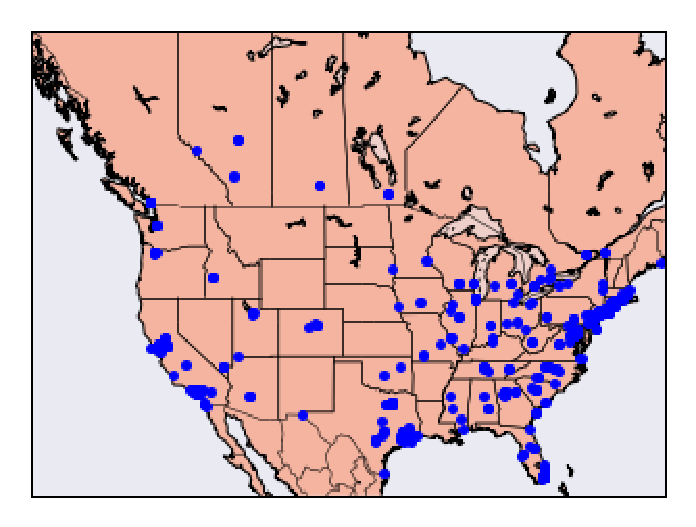
\includegraphics[height=2.5in, width=3.5in]{map}
\caption{Plot of geolocated tweets.}
\end{figure}

\subsection{Word and Document Similarity}

% show text of relevent tweets from d2v

% talk a bit about pre processing

The first analyses that we performed sought to identify certain keywords, hashtags, tweets and users, that were discussing HIV and PrEP related contexts. Word2Vec and the related method, Paragraph2Vec are unsupervised machine learning methods that have performed well at embedding natural language in a semantic vector space. In our analysis, Word2Vec allows us to determine semantically similar words, while Paragraph2Vec allows us to determine similar tweets, users and hashtags.



% table 1 - w2v PrEP
\begin{table}
\centering
\caption{Cosine Similarity to 'truvada'}
\begin{tabular}{|l|c|} \hline
Related Word & Cosine Similarity to 'truvada'\\ \hline
truvada & 0.796666\\ \hline
Truvada & 0.793999\\ \hline
DoingIt & 0.738141\\ \hline
WorldAidsDay & 0.728808\\ \hline
WorldAIDSDay & 0.720910\\ \hline
NancyReagan & 0.717667\\ \hline
NBHAAD & 0.705061\\ \hline
ART & 0.704300\\ \hline
hiv & 0.702844\\ \hline
HLM2016AIDS & 0.698698\\ \hline
\hline\end{tabular}
\end{table}

% table 2 - d2v PrEP
\begin{table}
\centering
\caption{Cosine Similarity to '\#truvada'}
\begin{tabular}{|l|c|} \hline
Related Hashtag/Tweet & Cosine Similarity to '\#truvada'\\ \hline
\#lgbtmedia16 & 0.739128\\ \hline
\#hiv & 0.727602\\ \hline
\#whereisprep & 0.707165\\ \hline
\#truvada & 0.696113\\ \hline
\#hivprevention & 0.636068\\ \hline
702179860983189504 & 0.630055\\ \hline
user-711275699529764864 & 0.629254\\ \hline
708519265540907010 & 0.628778\\ \hline
712032637024653313 & 0.628646\\ \hline
\#harrogatehour & 	0.628547\\ \hline
\hline\end{tabular}
\end{table}

% show PCA for each table above (remember to mention percent varience)

\subsection{Time Domain}

% PrEP related trends (2 topic time series worth)
% World AIDs day as validation (1 topic time series)

Next we sought to identify some temporal trends in PrEP related trends. We used Dynamic Topic Modelling to identify how certain topics change over time. We specified 10 topics and plotted representative words from two of the topics.

In topic 3 we see that the keyword 'prep' remains relatively constant, while 'prevention' and 'truvada' decline over time. 'hivaids' increases and then decreases in magnitude over the course of the time series (Figure 2). These dynamics may indicate short term events in hivaids and PrEP-related conversation on twitter over the time period studied.

We found that topic 5 captured several keywords related to World AIDS Day (Figure 3). We can see that all of these terms peak in the 47th week of 2015 and then decline into 2016. This correlates well with the actual date of World AIDS Day, December 1st. While we aren't specifically interested in World AIDS Day to inform our understanding of PrEP discussion, this observation validates our ability to identify temporal events using DTM.

% figure 2
\begin{figure}
\centering
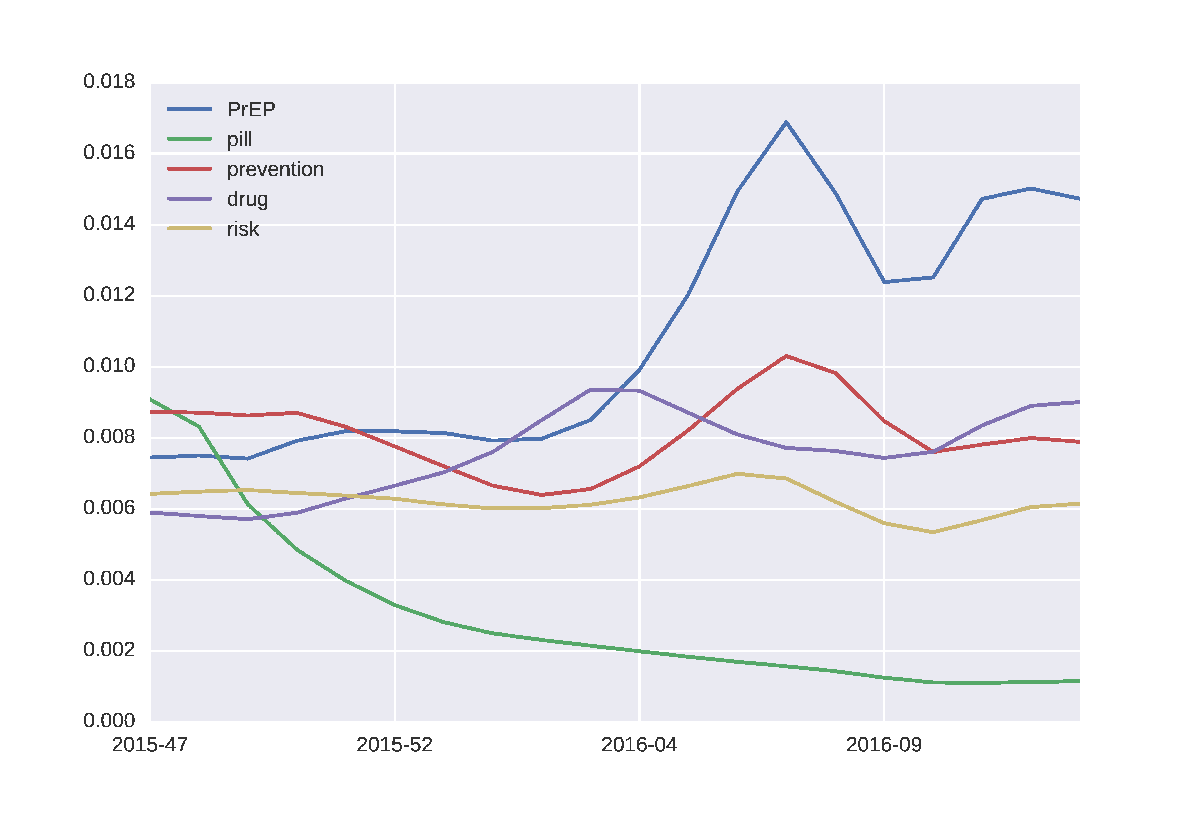
\includegraphics[height=2.5in, width=3.5in]{DTMfig1}
\caption{DTM topic 3 word prevalence over time. Date is YYYY-WW.}
\end{figure}

% figure 3
\begin{figure}
\centering
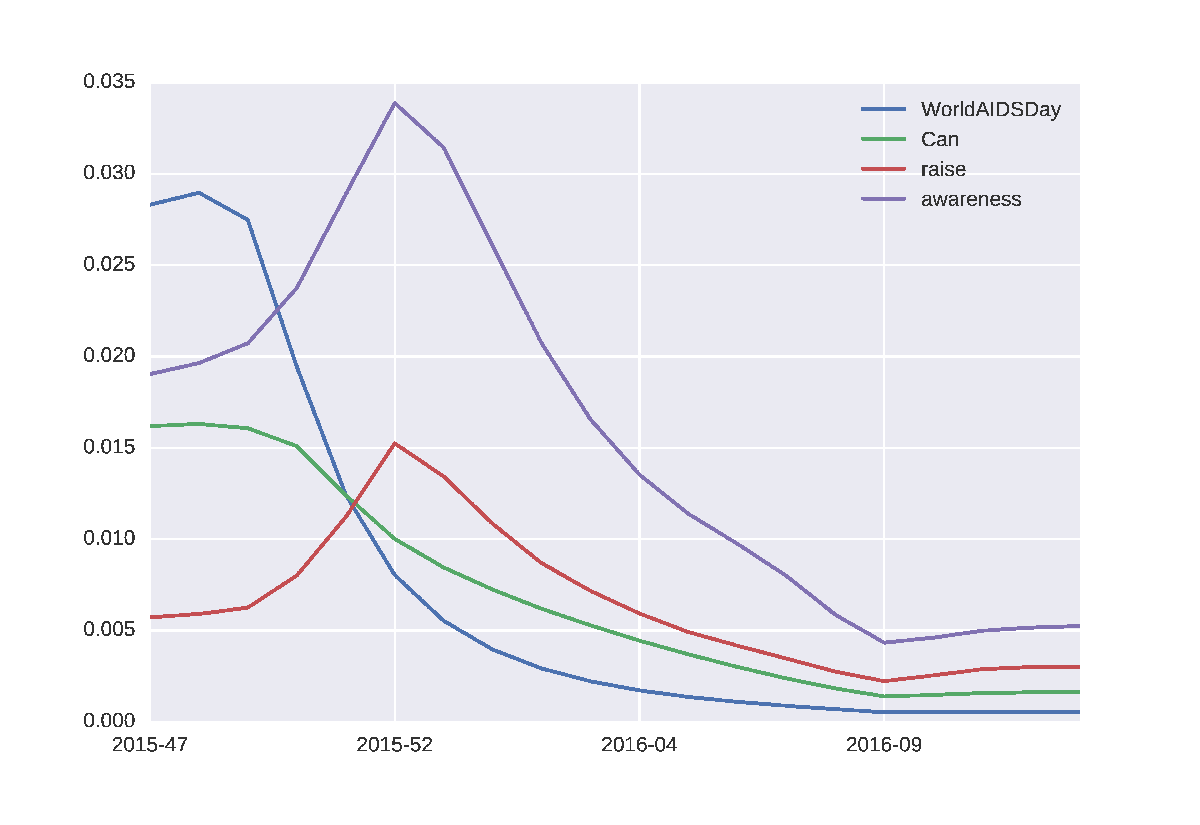
\includegraphics[height=2.5in, width=3.5in]{DTMfig2}
\caption{DTM topic 5 word prevalence over time. Date is YYYY-WW.}
\end{figure}

\subsection{User Timeline Analysis}

 this will take time to complete (running download, prob 5 days, so approx April 19th)

1 figure (heatmap of users vs topics)

1 table (top words for 10 topics)

\subsection{Sentiment Classification}

% top positive and negative example tweets
% report accuracy
% (potentially) report topic modeling on top postive and negative PrEP tweets

Lastly we sought to create a classification scheme to classify the sentiment of tweets either positive or negative. This classifier would allow us to quickly identify positive and negative PrEP related tweets to guide public health efforts. We first performed Paragraph2Vec on both our PrEP related tweet corpus and on another tweet corpus that had binary sentiment labels, positive, or negative. Then we trained a simple logistic regression classifier on the paragraph-vectors. We found that our classifier had an accuracy of 70\% on a validation set.

We then used this classifier to classify our PrEP related tweets into positive or negative labels. We reported the most positive, and most negative tweets, by log(probability), on our full dataset, and on tweets that specifically mention either 'prep' or 'truvada' (Table 4). It seems that overall the classifier seems to capture the sentiment relatively well, however it clearly fails to recognise the sarcasm present in the most positive overall tweet.

The sentiment results aren't perfect, but they do help us identify positive individuals in PrEP and HIV public health such as user @greg0wen. The sentiment tweets also let us uncover some of the prevailing stigmas and negative sentiments surrounding PrEP usage.

% do a top positive tweets table

% do a top negative tweets table


\section{Conclusions}

Conclusions go here.

Example citation (needed right now to compile):\cite{Lamport:LaTeX}

%\end{document}  % This is where a 'short' article might terminate

%ACKNOWLEDGMENTS are optional
\section{Acknowledgments}

Acknowledgements (optional) go here.

%
% The following two commands are all you need in the
% initial runs of your .tex file to
% produce the bibliography for the citations in your paper.
\bibliographystyle{abbrv}
\bibliography{sigproc}  % sigproc.bib is the name of the Bibliography in this case
% You must have a proper ".bib" file
%  and remember to run:
% latex bibtex latex latex
% to resolve all references
%
% ACM needs 'a single self-contained file'!
%
% no appendix for now...


\subsection{References}




\end{document}
